\section{Evaluation}

We conducted a 10-subject exploratory study to better understand how accelerators could help programmers during code modification tasks.
We had the following goals in mind:
\begin{enumerate}
\item Assess whether \gls{name}-generated explanations were readable and relevant for a set of code modification tasks.
\item Understand what information in an accelerator was most useful to programmers and what information was extraneous.
\item Determine when our accelerators failed to help users complete code modification tasks, and where they turned for help when context-relevant explanations were not available.
\end{enumerate}

\andrew{Update the numbers below based on final figures.}
We recruited 10 programmers from U.C. Berkeley listservs targeted to undergraduate and graduate students in computer science and information science.
In a screening survey, we verified that subjects had at least one year of programming experience.
Programmers had spent a median of 3 years in their longest-used language.
During warmup activities, 5 could accurately complete all 3 web programming tasks testing knowledge of HTML, CSS and Javascript, and 4 could correctly produce command lines for UNIX command lines \texttt{ls}, \texttt{wget}, and \texttt{grep}.

Each subject performed 8 code modification tasks in two languages for which we developed \glspl{name}: CSS selectors and \texttt{wget}.
Subjects were shown a 1-minute video on the thinkaloud protocol and asked to speak aloud about what problems they were solving, how they were solving it, and why they chose the strategies they did.

Each code modification task comprised three steps.
First, she read a task they had to perform --- e.g., \emph{write a CSS selector that selects only elements of class \texttt{myInput}.}
Second, she viewed a snippet that contained some clue of how to perform the task.
For example, see Figure~\ref{fig:study_snippet}, where a user is shown a snippet containing CSS selectors that chooses elements of class \emph{myCheckbox} without explaining the syntax of the selector.
On every other task, we asked the subject to find all explainable code fragments in the snippet and view their accelerators.
This ordering was counterbalanced across subjects.
After viewing the snippet and the accelerator, subjects were told they could use any resources they wanted, including the web, in order to solve the problem.
Third, she tested her code in a testbed we provided to assess it for correctness.
This allowed the subject to compare her output to expected output and rework her command until it was correct.
In general, subjects were given 5 minutes to complete all tasks, in the interest of time.
However, in some situations where subjects had extra time and they had not yet completed the tasks, we asked them to continue so we could observe their problem-solving process.

\begin{figure}
\centering
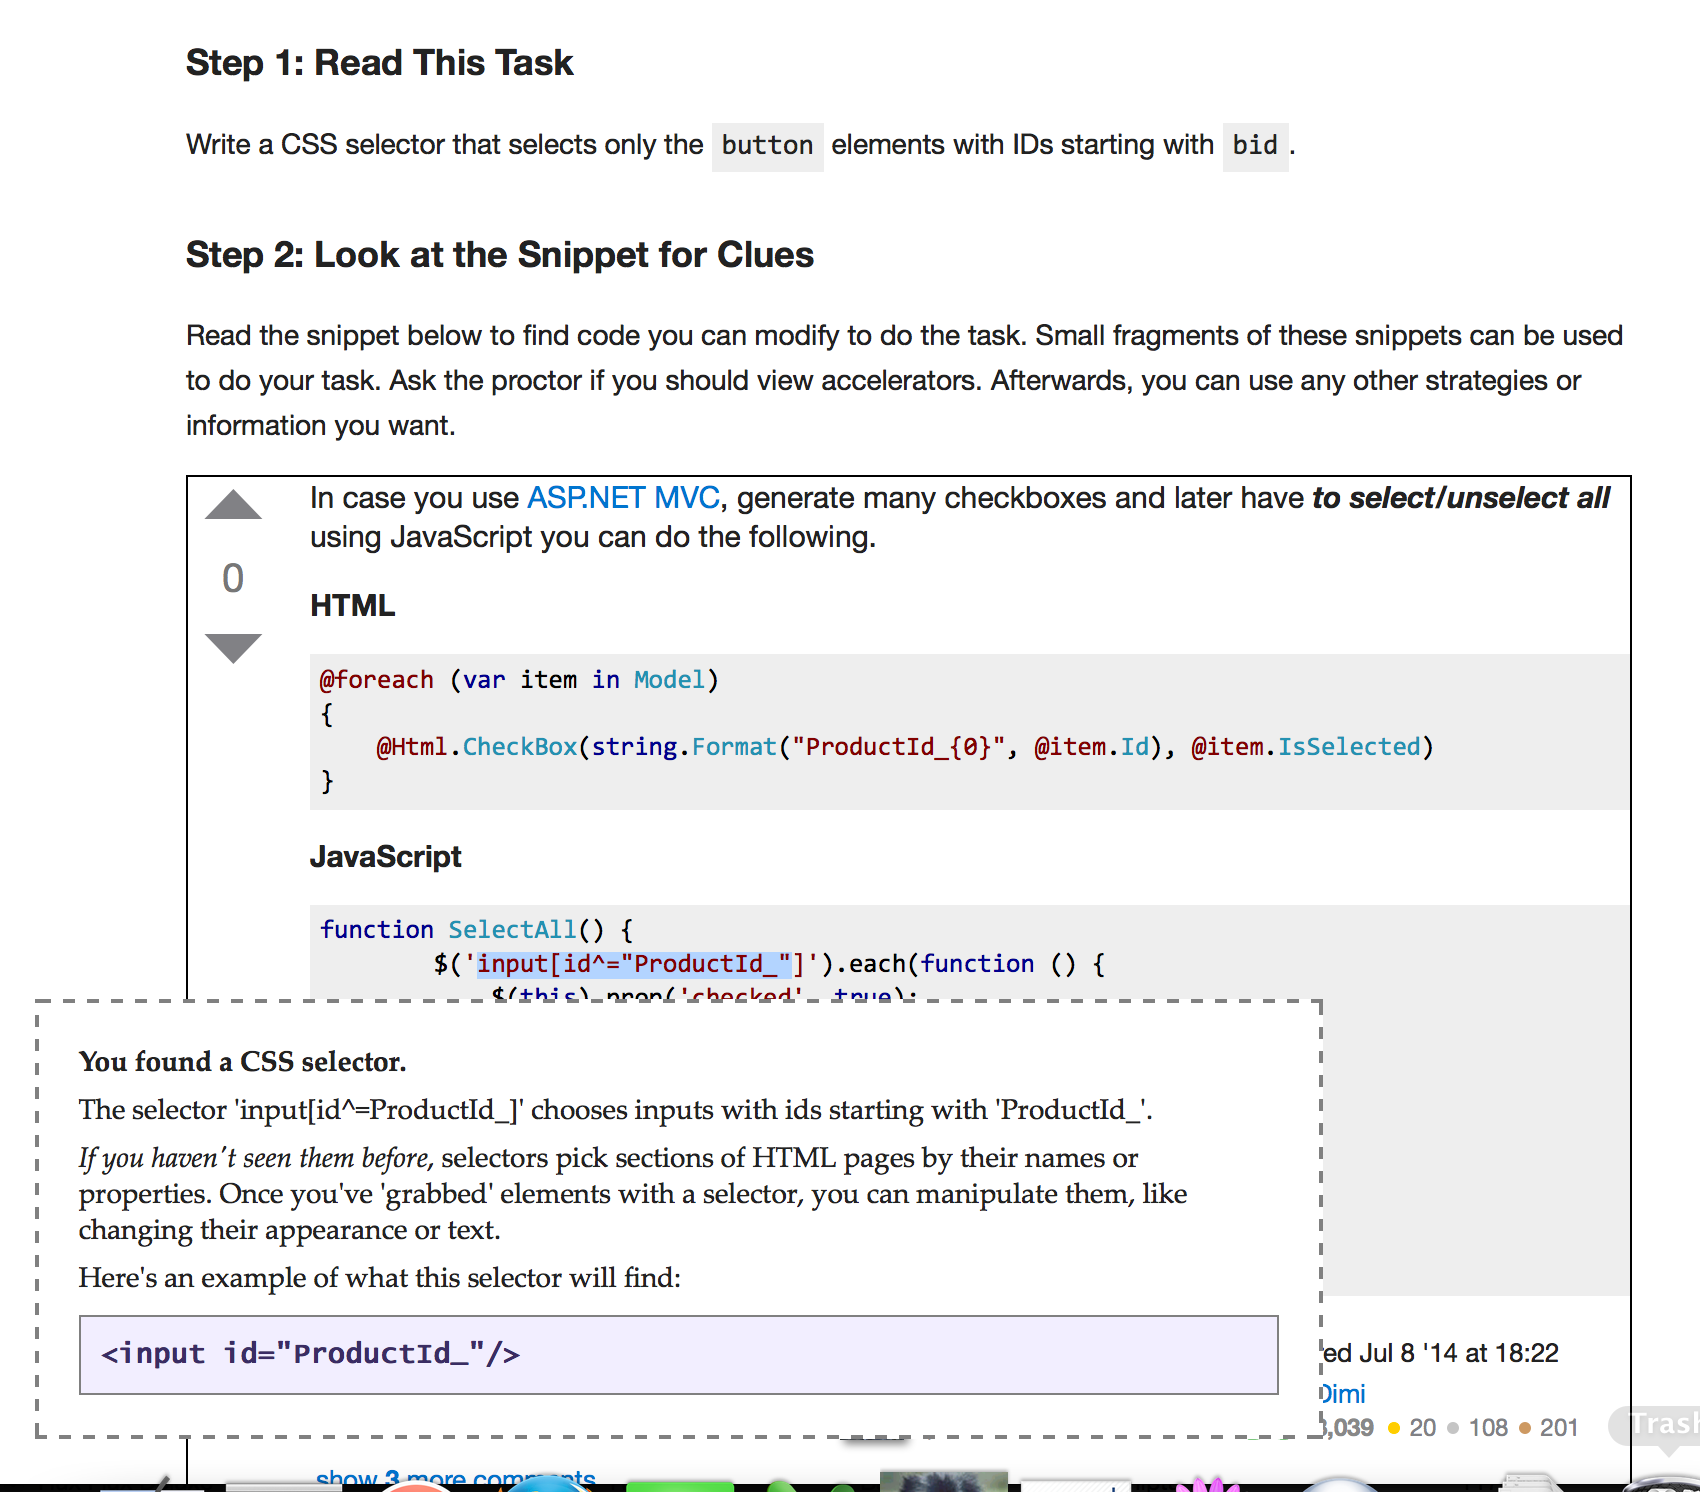
\includegraphics[width=0.4\textwidth]{figures/study_snippet}
\caption{An example snippet shown as a clue for a code modification task.}
\label{fig:study_snippet}
\end{figure}

In the space below, we discuss findings about the usability and utility of automatically generated accelerators in code modification tasks.
We refer to our twelve subjects by names $U{1-10}$.

\subsection{Accelerators Help Programmers Modify Code}

Automatic descriptions and demonstrations of CSS selectors and wget commands helped programmers solve the code modification tasks.
For the most complex CSS selector task, two of our subjects told us that the example HTML shown in the accelerator provided them with a pattern of what fields needed to be changed in from the selector in the snippet to capture the element and ID required by the task prompt ($U2$, $U4$).
Subjects were able to identify what flags had to be removed from wget commands without consulting external documentation, despite not having used the wget before ($U4$).
For others, the accelerator affirmed a guess that the subject already had about how to construct a CSS selector ($U1$).
For another subject with little previous experience with CSS selectors, an accelerator in an earlier task provided him with the knowledge needed to write the selector for the next two tasks, one task for which he was not allowed to view accelerators ($U5$).
One benefit of the accelerators, one user claimed, was that sometimes they closely matched the wording of the task prompt, making it easy to map flags for the wget command line to the higher-level intent of the task ($U4$).

Despite this evidence that accelerators can provide relevant information in code modification tasks, we note that the automatically-generated explanations were not always helpful, for several reasons.
First, there weren't always accelerators for the code fragments users wanted to have explained --- for instance, $U2$ thought that viewing an explanation for the \texttt{.prop} method of a jQuery selection would better steer him towards learning about a CSS selector for choosing elements of a specific class, but no explanation appeared when he selected the text of the method.
Second, programmers may fail to find the code for which accelerators will provide the key insight for the task.
While $U2$ eventually found a snippet that led him to writing a successful CSS selector for the fourth CSS task, he stumbled upon it randomly when reminded that he hadn't viewed all the accelerators in the snippet ($U2$).
Third, accelerator text may not be verbose enough to prevent programmers from developing inadequate mental models of new languages.
Even after all 4 CSS selector tasks, $U5$ appeared to believe that CSS selectors were HTML elements themselves, rather than labels that could fetch them, perhaps confused by the example HTML docs produced in each accelerator ($U5$).
The same user described \texttt{wget}'s recursive method as descending through directories instead of links ($U5$).
Fourth, programmers may not carefully read text descriptions of code in an accelerator.
Two subjects admitted to skimming over or ignoring the second sentence in every CSS selector accelerator which introduces the purpose of a CSS selector ($U3$,$U4$).
One subject that clearly uttered the text of the full CSS selector accelerators several times as he read them claimed that he likely could have improved his understanding of what a CSS selector was by reading this text more carefully ($U5$).
Fifth, some programmers felt that the \gls{name}-generated explanations were not enough.
$U3$ told us that she wanted to see authoratative documentation from the developers of the language, and asked that we link to it from the accelerator ($U3$).

\subsection{Usage Patterns for Activating Accelerators}

Programmers access accelerators by selecting code fragments on the page that they want to have explained.
No users reported a difficult experience getting to learn how to show an accelerator for a code fragment.
In addition, we noted that many of the users selected text when walking through the code during think aloud.
Three subjects selected code in tasks where accelerators were disabled when describing either thinking about the code or describing it to the study proctor ($U2$, $U4$, $U5$).
One subject even inadvertently brought up an accelerator while pointing out code to the proctor ($U1$).
We believe that for some participants, activating the accelerators by selecting text became a natural, instinctual action.
In the final wget task, on subject selected text for a flag he didn't know before remembering that accelerators were turned off for the task ($U5$).
Many subjects tried to activate accelerators to describe single arguments of wget commands ($U2$, $U3$, $U4$, $U5$).
This worked in their cases, as there was only ever one code snippet on the page to be explained, and the substring they chose matched the explainable code fragment according to our selection algorithm.

However, the leniency of our algorithm for matching a text selection to an explained code fragment caused confusion for programmers about what fragments would be explained on each page ($U1$, $U2$, $U5$).
For the same reason, explanations generated did not always match the fragment selected ($U1$, $U3$, $U5$).
For example, one user selected the text \texttt{<p>} for which no explanation was generated by the explanation server, as no CSS selector starts with a less-than sign.
However, our selection matching algorithm matched this string to the \texttt{p.mainPageMeters} selector for which an explanation \emph{had} been generated by the server.
As a result, this user viewed an irrelevant explanation for the code fragment he was viewing ($U5$).

\subsection{Problem-Solving Strategies when Accelerators Were Missing}

We noticed several strategies that programmers drew upon to solve problems when their personal knowledge was insufficient for completing the code modification task and accelerators were deactivated.
We mention them here to emphasize the effort required when authoratative explanations of code is not within immediate reach.

First, we found that most users in at least one task adopted a try-it-first workflow.
As $U2$ descrcibed, reasoning about the task and the code may be more powerful than attempting to understand possibly irrelevant context of related code snippets from StackOverflow.
During early CSS selction tasks, $U1$ preferred to attempt a selector prior to viewing the code snippet for clues.
$U4$ expected that the \texttt{div.cont} selector would work for the third CSS task and decided she would try the selector before looking for documentation that could confirm if this was the best selector.
She also referred to her own methods as `guess-and-check' when she continually compared the output of her wget command to the test output we provided when determining if her command was correct.
Similarly, $U5$ told us that he was tempted to see if his first guess of CSS selector worked for the final CSS task before incorporating any of the new syntax shown in the code snippet.
In the \texttt{wget} tasks, the same user performed trial and error by removing options and seeing if the output matched what he expected, instead of taking the time to understand the meaning of each flag by consulting documentation ($U5$).

All of our users at some point accessed documentation to gain more information about the code they were working with.
Several accessed the UNIX man pages on wget ($U1$, $U2$, $U3$).
Two turned to Google instead of the man pages for help on wget, but both users ended up at some point on the online man page for the command ($U4$, $U5$).
One user transitioned from the man pages to Google when she found that the man page had unhelpful descriptions of flags ($U3$).
For finding help on CSS selectors, two users started with a Google search, and eventually ending up at the jQuery documentation ($U3$) and the other finding what they believed to be a clear, simple solution on StackOverflow ($U5$).
The challenges of working with this documentation was enough to merit the next subsection.

We found that programmers would rely on past knowledge for problem-solving in several ways.
At least two subjects admitted to adapting patterns from solutions to previous tasks, sometimes sucessfully ($U4$) and sometimes unsuccessfully ($U5$).
One programmer actually referenced code used in a previous task when debugging an error in a later task ($U4$).
Programmers drew connections to previous knowledge to find insights for fragments to inspect and code to write.
$U1$ thought that the syntax of \texttt{input[id\^=...]} appeared familiar for string matching.
$U5$ justified his use of the '\texttt{.}' symbol for selecting elements of a particular class by comparing this to specifying properties in Java.
In another case, $U5$ unsuccessfully attempted to use the (nonexistent) \texttt{-f} flag to force re-downloading of files for wget, recalling that this flag is used in other UNIX commands to force the transfer of files.

\subsection{Challenges Using Conventional Programming Help}

Some programmers had difficulty searching for programming help on Google and using the results.
One subject could not express the symbols '\texttt{\^=}' as query term when searching for affirmation about what this pattern signifies in CSS selectors.
Her follow-up queries with English language query terms only were so vague that the top results were irrelevant to describing these symbols that the subject wanted to learn about ($U3$).

Programmers also found conventional forms of programming help difficult to navigate.
When searching for the \texttt{-r} flag in both the Terminal-based ($U2$) and browser-based ($U4$) man page for wget, subjects found that an internal document search for the flag yielded so many matches that it was difficult to find the actual definition of the flag.
The portion of the description of the \texttt{-N} timestamp flag that was relevant to the code modification task was not placed directly adjacent to where the flag was introduced, so one subject missed this information, even though it was only 10 lines away ($U3$).

Many subjects showed some wrong conceptual model of what code in a snippet or their solution actually did.
$U1$ appeared to believe that IDs were typically referred to by the \texttt{[id=]} pattern instead of by a simple \texttt{\#}.
$U3$ assumed that wget downloaded files recursively from a URL by default, and also believed that jQuery was the authoratative source on the '\texttt{\^=}' syntax in CSS selectors, whereas it's really part of standard CSS.
Some users made more than one faulty assumption.
$U4$ assumed after looking at documentation that Terminal commands might be case insensitive, so she assumed that the \texttt{-R} and \texttt{-r} flags were the same flag.
During the final task, she believed that the \texttt{-p} flag was used to download directories instead of a flat hierarchy.
This points to the necessity to provide the appropriate in-situ help to ensure that users can overcome potentially dangerous assumptions when working with new code.

In a couple of cases, users failed to notice a critical error in their code that could be solved by a trivial fix from a close inspection.
$U4$ spent some time attempting to find an option to download directories from a URL, when in fact the problem was that a \texttt{/} was missing from the end of the URL.
$U5$ assumed he had removed the \texttt{-p} flag from his command and was confused why it was still downloading images, until some close inspection later revealed that it had not been removed.
Future in-situ help should assist programmers detect such trivial errors.

This affirms the value of \gls{name} as in-situ explanations of code.
Future studies can determine the frequency that novice and end-user programmers seek additional information for solving code modification tasks.

\subsection{Threats to Validity}

In the future, we are interested in conducting our study with groups of specifically novice programmers.
While we believe the findings we have presented about accelerators in this paper are legitimate, we believe that viewing the problem-solving strategies of novice programmers in particular will yield better recommendations for how to design in-situ help for this group.
